%!TEX root = thesis.tex

\cleardoublepage
\thispagestyle{plain}

\pdfbookmark{Abstract}{abstract}
\paragraph{Abstract}
Don't Copy That Floppy was an anti-copyright infringement campaign run by the Software Publishers Association (SPA) beginning in 1992.\cite{Edg03} The video for the campaign, starring M. E. Hart as "MC Double Def DP," was filmed at Cardozo High School in Washington, D.C. and produced by cooperation between the SPA, the Educational Section Anti-Piracy Committee, and the Copyright Protection Fund, in association with Vilardi Films. The groups distributed the film for general viewing through VHS tapes that were mailed to schools. In later years, the film became a viral video sensation through websites such as YouTube, where the official page has had over 1,000,000 views as of December 2013.

In May 2009, the Software and Information Industry Association (formed in 1999 when the Software Publishers Association merged with the Information Industry Association) released the trailer for a follow-up to Don't Copy That Floppy, called Don't Copy That 2, released on September 9, 2009. The sequel features MC Double Def DP as he continues his crusade against "piracy" in the digital age.

\begin{figure}
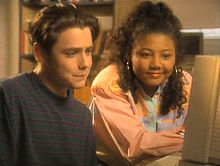
\includegraphics{220px-Dontcopythatfloppy3.jpg}
\caption{Screenshot from ad showing Corey and Jenny playing a video game.}
\label{fig:kids}
\end{figure}

\cleardoublepage
\thispagestyle{plain}

\foreignlanguage{german}{%
\pdfbookmark{Kurzfassung}{kurzfassung}
\paragraph{Kurzfassung} 
 ''Don't Copy That Floppy'' war eine Kampagne gegen Urheberrechtsverletzungen der Software Publishers Association (SPA), welche 1992 begann. Das Video zur Kmpagne, mit M. E. Hart in der Hauptrolle als ''MC Double Def DP'', wurde in der Cardozo High School in Washington, D.C.  gefilmt. Es wurde produziert von einer Kooperation zwischen SPA, dem Educational Section Anti-Piracy Committee, dem Copyright Protection Fund, in Zusammenarbeit mit Vilardi Films. The gruppen verteilten den Film zur Vorführung auf VHS-Kassetten, welche an Schulen verschickt wurden. Einige Jahre später wurde der Film zum viralen Hit auf Video-Streming Seiten wie Youtube, wo die offizielle Seite im Dezember 2013 über 1 Mio. Aufrufe hatte. \\ 
  Im Mai 2009 veröffentliche die the Software and Information Industry Association (entstanden 1999, als sich die Software Publishers Association mit der Information Industry Association zusammenschloss) einen Trailer für einen Nachfolger zu Don't Copy That Floppy, Don't Copy That 2, welcher am 9.September 2009 erschien. Der Nachfolger zeigt, wie MD Couble Pref seinen Kreuzzug gegen Internet-Piraterie im digitalen Zeitalter fortsetzt.
}